%Dokumentinnstillinger:---------------------------------
\documentclass[11pt,norsk]{elsys-design}


\heading{Designnotat} 
\title{Tittel}
\author{Forfatter Forfattersen}
\version{1.0}
\date{\today}

\begin{document}

\maketitle

%Automatisk generert innholdsfortegnelse:------------------
\toc

%Selve rapporten:------------------------------------------
\section{Problembeskrivelse}
\label{sec:innledning}

Se word-versjonen av designnotat-malen for beskrivelse av hva som skal være med i de forskjellige delene.

\section{Prinsipiell løsning}
\label{sec:prinsipielllosning}

Blablabla. Løsningen er basert på kretsen i~\cite[s. 1604]{bibelen}. Slik som dette refererer vi altså til bibliografien. Videre ser vi av formelen
\begin{equation}
	\label{eq:formel}
	x = \frac{-b \pm \sqrt{b^{2}-4ac}}{2a}
\end{equation}
at dette kommer til å bli meget bra. Vi kan også referere til likning (\ref{eq:formel}) igjen.

\section{Realisering og test}
\label{sec:realisering}

Målinger av $v_1$ og $v_2$ er vist i figur~\ref{fig:resultat}.
\begin{figure}[htbp]
	\centering
	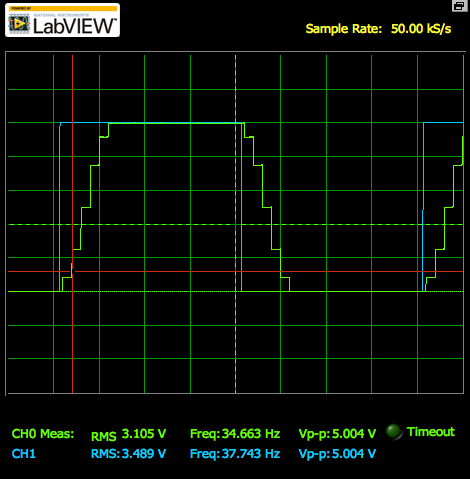
\includegraphics[width=0.45\textwidth]{skop} 
	\caption{Inngang $v_1$ (blå kurve) og utgang $v_2$ (grønn).}
	\label{fig:resultat}
\end{figure}

Slik setter vi altså inn en figur og refererer til den. 

Vi kan også kryssreferere til f.eks. seksjon~\ref{sec:prinsipielllosning} ved å bruke labels.



\section{Konklusjon}
\label{sec:konklusjon}

Blablabla. ... som er innenfor 10\% av kravet.

\section{Takk}
Blablabla.

%Bibliografi: Legg til flere elementer ved å legge til flere \bibitem:--------
\phantomsection
\addcontentsline{toc}{section}{Referanser}
\begin{thebibliography}{99}

\bibitem{bibelen}
	Albert Einstein,
	\emph{Elektronikkbibelen},
	O Store Forlag,
	1. utgave,
	1930.

\end{thebibliography}

\appendix
%Tillegg. Flere tillegg legges til ved å lage flere sections:-----------------
\section{Ekstra greier}
Mindre relevant blabla.


\end{document}